% --- Template for thesis / report with tktltiki2 class ---
% 
% last updated 2013/02/15 for tkltiki2 v1.02

\documentclass[finnish]{tktltiki2}

% tktltiki2 automatically loads babel, so you can simply
% give the language parameter (e.g. finnish, swedish, english, british) as
% a parameter for the class: \documentclass[finnish]{tktltiki2}.
% The information on title and abstract is generated automatically depending on
% the language, see below if you need to change any of these manually.
% 
% Class options:
% - grading                 -- Print labels for grading information on the front page.
% - disablelastpagecounter  -- Disables the automatic generation of page number information
%                              in the abstract. See also \numberofpagesinformation{} command below.
%
% The class also respects the following options of article class:
%   10pt, 11pt, 12pt, final, draft, oneside, twoside,
%   openright, openany, onecolumn, twocolumn, leqno, fleqn
%
% The default font size is 11pt. The paper size used is A4, other sizes are not supported.
%
% rubber: module pdftex

% --- General packages ---

\usepackage[utf8]{inputenc}
\usepackage[T1]{fontenc}
\usepackage{lmodern}
\usepackage{microtype}
\usepackage{amsfonts,amsmath,amssymb,amsthm,booktabs,color,enumitem,graphicx}
\usepackage[pdftex,hidelinks]{hyperref}
\usepackage{tikz}
\usepackage{graphicx}
\usepackage{caption}
\usepackage{subcaption}
\usepackage{amsmath}
\usepackage{todonotes}


% Automatically set the PDF metadata fields
\makeatletter
\AtBeginDocument{\hypersetup{pdftitle = {\@title}, pdfauthor = {\@author}}}
\makeatother

% --- Language-related settings ---
%
% these should be modified according to your language

% babelbib for non-english bibliography using bibtex
\usepackage[fixlanguage]{babelbib}
\selectbiblanguage{finnish}

% add bibliography to the table of contents
\usepackage[nottoc]{tocbibind}
% tocbibind renames the bibliography, use the following to change it back
\settocbibname{Lähteet}

% --- Theorem environment definitions ---

\newtheorem{lau}{Lause}
\newtheorem{lem}[lau]{Lemma}
\newtheorem{kor}[lau]{Korollaari}

\theoremstyle{definition}
\newtheorem{maar}[lau]{Määritelmä}
\newtheorem{ong}{Ongelma}
\newtheorem{alg}[lau]{Algoritmi}
\newtheorem{esim}[lau]{Esimerkki}

\theoremstyle{remark}
\newtheorem*{huom}{Huomautus}


% --- tktltiki2 options ---
%
% The following commands define the information used to generate title and
% abstract pages. The following entries should be always specified:

\title{Madonreiät langattomissa ad hoc -verkoissa}
\author{Jan Wikholm}
\date{\today}
\level{Kandidaatintutkielma}
\abstract{Madonreikähyökkäysten ja niiden vastatoimien tyypitys.}

% The following can be used to specify keywords and classification of the paper:

\keywords{ad hoc -verkot, wlan, hyökkäys, puolustus, havainnointi}

% classification according to ACM Computing Classification System (http://www.acm.org/about/class/)
% This is probably mostly relevant for computer scientists
% uncomment the following; contents of \classification will be printed under the abstract with a title
% "ACM Computing Classification System (CCS):"
% \classification{}

% If the automatic page number counting is not working as desired in your case,
% uncomment the following to manually set the number of pages displayed in the abstract page:
%
% \numberofpagesinformation{16 sivua + 10 sivua liitteissä}
%
% If you are not a computer scientist, you will want to uncomment the following by hand and specify
% your department, faculty and subject by hand:
%
% \faculty{Matemaattis-luonnontieteellinen}
% \department{Tietojenkäsittelytieteen laitos}
% \subject{Tietojenkäsittelytiede}
%
% If you are not from the University of Helsinki, then you will most likely want to set these also:
%
% \university{Helsingin Yliopisto}
% \universitylong{HELSINGIN YLIOPISTO --- HELSINGFORS UNIVERSITET --- UNIVERSITY OF HELSINKI} % displayed on the top of the abstract page
% \city{Helsinki}
%


\begin{document}

% --- Front matter ---

\frontmatter      % roman page numbering for front matter

\maketitle        % title page
\makeabstract     % abstract page

\tableofcontents  % table of contents

% --- Main matter ---

\mainmatter       % clear page, start arabic page numbering

\section{Johdanto}

% Write some science here.


Langattomat päätelaitteet -- kuten matkapuhelimet, PDA:t ja kannettavat tietokoneet -- voivat muodostaa langattoman ad hoc -verkon, jonka avulla ne voivat kommunikoida ilman erillistä verkkoinfrastruktuuria \cite{delphi}. Sensori- ja ad hoc -verkot voivat toimia viestintäalustana monissa erilaisissa käyttötarkoituksissa kuten pelastus-, armeija- \cite{leashes} sekä  siviilikäytössä \cite{liteworp}. Esimerkiksi luonnonkatastrofin jäljiltä perinteiset langattomat tukiasemat voivat olla tuhoutuneet ja täten pelastuslaitosten työntekijät ovat viestinnässään ad hoc -verkkojen varassa \cite{leashes}.

\noindent \\
Näiden verkkojen suurimpia etuja ovat käyttöönoton nopeus ja kustannustehokkuus \cite{delphi,leashes}, sillä laitteisto on usein edullista ja päätelaitteet osaavat itsenäisesti luoda verkon. Vaikka ad hoc -verkkoja voi muodostaa myös langallisesti, on useimmiten käytössä langattomat teknologiat \cite{leashes} ja siksi keskitymme niihin.

\noindent \\
Pääosa ad hoc -verkkojen alkuvaiheen tutkimuksesta on keskittynyt verkkojen itsenäiseen käyttöönoton parantamiseen ja laitteistovaatimusten pienentämiseen luoden reititysprotokollia ja muita välttämättömiä viestinnän osia \cite{liteworp}. Ad hoc -verkkojen avoimuuden ja autonomisuuden seurauksena ne ovat erityisen haavoittuvia monille erilaisille hyökkäyksille: \emph{salakuuntelu} (eavesdropping), \emph{väärennys} (spoofing) ja \emph{toistaminen} (replay) \cite{leashes}. Näiden lisäksi hyökkääjä voi tahallisesti olla välittämättä paketteja, jota kutsutaan \emph{musta aukko -hyökkäykseksi} (blackhole attack), tai syöttää niitä verkkoon paljon tukehduttaakseen sen järkevän käytön, jota kutsutaan nimellä \emph{valkoinen aukko -hyökkäys} (white hole attack) \cite{delphi}. \emph{Madonreikähyökkäys} (wormhole attack) on erityisen vakava hyökkäys ad hoc -verkoissa \cite{liteworp}.

\noindent \\
Madonreikähyökkäyksessä yleensä kaksi tai useampi paha-aikeista tahoa toimivat yhteistyössä saadakseen liikenteen ohjautumaan niiden välillä kulkevaa reittiä pitkin, jotta voivat toteuttaa yllä lueteltuja hyökkäyksiä. Nämä tahot välittävät kaikki kuulemansa paketit toiselle osapuolelle, joka toistaa ne omassa päässään. Tämä pakettien välitys voidaan toteuttaa hyökkääjien omalla suurinopeuksisella tiedonsiirtokanavalla, pakettien kapseloinnilla normaalia verkkoa pitkin tai vaikka suuritehoisella lähettimellä \cite{liteworp}. Tunnelin ollessa toiminnassa se häiritsee reititysprotokollia tarjoten lyhimmän ja yleensä nopeimman reitin, joten muut verkon laitteet päätyvät lähettämään suuren osan paketeista sen läpi. 

\noindent \\
Madonreikähyökkäyksen toiminta perustuu nimenomaan ad hoc -verkkojen määrittävään ominaisuuteen -- niiden autonomiseen reititykseen. Tukiasemiin perustuvassa verkossa vastaava ei voi toimia, koska kaikki liikenne ohjataan aina tukiasemien kautta.

\noindent \\
Erityisen salakavalan hyökkäyksestä tekee se, että hyökkääjien ei tarvitse murtaa mitään salausta koska koko hyökkäys perustuu pakettien kopiointiin (salakuunteluun ja sen jälkeiseen toistoon) verkon osasta toiseen.

\noindent \\
Esittelemme luvussa 2 madonreikähyökkäysten hyökkääjä- \cite{delphi} ja hyökkäystyypit \cite{liteworp}, minkä jälkeen kerromme laitteistoriippuvaisista puolustuskeinoista luvussa 3 ja protokollapohjaisista puolustuksista luvussa 4.


\section{Hyökkääjä- ja hyökkäystyypit}

Madonreikähyökkääjiä on kahta eri tyyppiä: \emph{piilotettu} ja \emph{avoin} \cite{delphi} ja hyökkäyksiä on viittä eri tyyppiä. \cite{liteworp}. Kaikkia hyökkäystyyppejä ei ole käsitelty kaikissa puolustuskeinoissa, joten käsittelemättömien hyökkäystyyppien torjumisen toimivuus on erinomainen kohde jatkotutkimukselle.

\subsection{Hyökkääjätyypit}
\paragraph{Piilotetut hyökkääjät} toimivat verkossa kertomatta muille verkon laitteille omasta olemassaolostaan. Ne kuuntelevat liikennettä ja siirtävät paketteja madonreiän läpi täysin muokkaamatta. Tällöin kaukanakin olevat laitteet voivat luulla madonreiän läpi tulevia paketteja naapureilta tuleviksi, koska eivät tiedä välissä olevan toistimena toimiva madonreikä.

\noindent \\
Esimerkiksi pakettihihnat, jotka esitellään luvussa ~\ref{packetleashes}, toimivat piilotettuja hyökkääjiä vastaan.

\paragraph{Avoimet hyökkääjät} rekisteröityvät verkkoon kuten muutkin laitteet. Muille verkon laitteille näyttää siltä, että nämä laitteet ovat ensimmäisen asteen naapureita ja siten niiden kautta löytyvä lyhyt polku on täysin käypä vaihtoehto. Tapa, jolla madonreikä on muodostettu, on jokin alla kuvailluista viidestä hyökkäystavasta.

\subsection{Hyökkäystyypit}

\paragraph{Erilliskaistahyökkäys} on se hyökkäystyyppi, johon yleisimmin viitataan nimellä \emph{madonreikähyökkäys}. Mikäli hyökkääjillä on normaalin lähetyskaistan - esimerkiksi wlan-verkkon - lisäksi käytössä vaikkapa yksinkertaisesti kytketty ethernetverkko, voivat ne kommunikoida yleistä verkkoa nopeammin ja sen kantamaa pidemmälle. Tämä sotkee reititysprotokollia ja suuri osa paketeista päätyy kulkemaan hyökkääjien linkin läpi.

\paragraph{Pakettikapseloinnissa} hyökkääjät H1 ja H2 voivat käyttää jo olemassa olevaa verkkoa: H1 kuulee paketin ja luo uuden H2:lle suunnatun paketin, jonka sisältönä on sellaisenaan H1:n kaappaama paketti. Kun tämä kapseloitu paketti saavuttaa H2:n, se toistaa alkuperäisen sisällön sellaisenaan verkkoon, joten sen naapurit luulevat H1:n naapureiden olevan lähellä. Tämä ei vaadi hyökkääjien osalta mitään muista verkon laitteista poikkeavia resursseja.

\paragraph{Suurteholähetys} on malliesimerkki siitä, että hyökkääjille voi olettaa loputtomat resurssit toisin kuin muille verkon laitteille, joita nimenomaan yleensä yhdistää resurssien vähyys. Tässä hyökkäystyypissä hyökkääjälaite lähettää kaappaamansa reitityspaketit huomattavan suurella lähetysteholla ja täten saa aikaan sen itsensä lävitse kulkevan lyhimmän reitin. Tämä hyökkäys ei siis vaadi kahta osapuolta.

\paragraph{Pakettivälitys} -- kuten suurteholähetys -- ei vaadi hyökkääjäparia vaan sen voi suorittaa yksikin vihamielinen laite. Tässä hyökkääjä on kahden laitteen välissä välittäen paketteja jolloin nämä laitteet luulevat olevansa naapureita ja hyökkääjä niiden välissä voi suorittaa esimerkiksi salakuuntelua tai palvelunestohyökkäystä.

\paragraph{Protokollapoikkeamat} ovat paha-aikeisten laitteiden tahallista verkkoprotokollan rikkomista: esimerkiksi pakettitörmäysten estämiseksi tietyt protokollat vaativat reitityspakettien lähetyksessä pientä viivettä - paha-aikeinen laite voi täten lähettää paketit heti ja aiheuttaa tavallisille laitteille haittaa törmäyksillä. Toinen vaihtoehto on reitityspakettien lähettämättä jättäminen, jolloin verkon reititys ja polunetsintä eivät toimi oikein. Kummassakin tapauksessa hyökkääjä voi junailla toimensa siten, että suuri osa verkon liikenteestä päätyy reitittymään sen läpi.

\section{Laitteistoriippuvaiset puolustusmekanismit}

Alla kuvatut puolustusmekanismit eivät vaadi reititysprotokolliin muutoksia, mutta niillä on laitteistovaatimuksia.

\subsection{Pakettihihnat ja TIK-protokolla}
\label{packetleashes}
Yih-Chun Hu et al \cite{leashes} kuvailevat uuden mekanismin - \emph{pakettihihnat} (packet leashes) - ja sen kaksi eri varianttia: \emph{aikahihnan} (temporal leash) ja \emph{geohihnan} (geographic leash). Tässä hihnalla tarkoitetaan sellaista tietoa, jolla paketin enimmäiskantamaa voidaan rajoittaa. Tällaista tietoa ovat esimerkiksi paketin vanhenemista ilmaiseva aikaleima tai lähettäjän paikkatiedon ja paketin maksimietäisyyden yhdistelmä.

\noindent \\
Pakettihihnojen lisäksi he luovat uuden TIK-verkkoprotokollan, joka käyttää aikahihnoja madonreikiä vastaan.

\paragraph{Aikahihnat} 
\noindent \\
Aikahihnojen edellytyksenä on tarkka kellojen synkronointitarkkuus: muutaman mikrosekunnin tai jopa satojen nanosekuntien tarkkuus. Kaikkien laitteiden pitää myöskin olla tietoisia virhemarginaalin suuruusluokasta kahden laitteen välillä. Tällainen synkronointitarkkuus onnistuu esimerkiksi GPS:n avulla. Vaikka tarkkuusvaatimus on erittäin tiukka, on se kirjoittajien mukaan täysin hyväksyttävä ottaen huomioon madonreikähyökkäyksen vakavuuden.

\noindent \\
Aikahihnaa muodostaessa lähettäjä päättää enimmäispituuden lähetykselle ja laskee synkronoinnin virhemarginaalin huomioiden, kauanko valonnopeudella kulkevalla radiosignaalilla kestää sinne päätyä. Tämän avulla lähettäjä asettaa paketille vanhenemisajan, jonka jälkeen paketti on hylättävä. Viestien tunnelointi aiheuttaa viivettä niiden kulkiessa fyysisesti kauemmaksi. Tämän viiveen takia viesti ehtii vanhentua ja madonreiän toisella puolella olevat laitteet hylkäävät sen.

\noindent \\
Vaikka aikahihna on hihnatyypeistä tarkempi, on sen haasteena se, ettei lähettäjä tiedä aina tarkalleen omaa lähetysaikaansa, koska fyysisen kerroksen lähetysmekanismi voi joutua odottamaan vuoroaan. Täten on vaikeaa etukäteen luoda lähetysajankohtaan perustuvaa digitaalista allekirjoitusta. Tämän kirjoittajat ovat ratkaisseet kohta esiteltävässä TIK-protokollassa.

\paragraph{Geohihnat}
\noindent \\
Geohihnoja käytettäessä kaikkien verkon laitteiden pitää tietää oma sijaintitietonsa sekä niiden pitää pystyä synkronoimaan kellonsa muiden kanssa. Kellojen synkronointitarkkuus ei ole niin tärkeä seikka, koska laitteiden liikkumisvauhti suhteessa valonnopeuteen on marginaalinen.

\noindent \\
Geohihnan toiminta on hyvin yksinkertainen: laite tarkistaa onko sen oma sijainti alkuperäisessä paketissa määritellyn sallitun matkan päässä. Koska paketit allekirjoitetaan digitaalisesti, voi laite luottaa paikannustiedon olevan alkuperäiseltä lähteeltä. Toisin kuin pelkkä matkan pituuteen perustuva tarkistus geohihnat toimivat myös siinä tilanteessa, että madonreikä kuljettaa paketin jonkin esteen ohi.

\noindent \\
Geohihnoissa laitteet tietävät toistensa oletetun maksimiliikenopeuden, ja täten madonreikätunneloitu paketti voidaan tunnistaa ilkivaltaisen laitteen lähettämäksi, jos se lähettää verkkoon kaksi pakettia, joiden lokaatiotiedoissa on tapahtunut maksimiliikenopeutta nopeampaa liikettä edellyttävä muutos.

\paragraph{TIK-protokolla} 
\label{tik}
\noindent \\
Tärkeimpänä ominaisuutena koko aikahihnafunktion toiminnassa on aikaleimojen luotettavuus; leimat pitää pystyä todentamaan. Todentamisen toteuttamiseen kirjoittajat hylkäävät jaetut avaimet suoraan todeten niiden hallinnan olevan liian raskas operaatio. Toisena ideana on digitaalisen allekirjoituksen liittäminen jokaiseen pakettiin, jolloin jokaiselle laitteelle riittää yksi julkinen--yksityinen-avainpari ja jokaisen laitteen tarvitsee tietää vain tämä kaikkien julkisten avainten joukko. Digitaaliset allekirjoitukset kuitenkin yleensä perustuvat raskaaseen asymmetriseen kryptografiaan, joka ei sovi ad hoc –verkkojen oletettuun resurssivähyyteen.

\noindent \\
Symmetriseksi vaihtoehdoksi tarjotaan tiivisteistä koostuvaa binääripuuta (Merkle-tiivistepuu). Tiivisteiden hyväksi puoleksi kerrotaan niiden erittäin tehokas laskeminen ja yksisuuntaisuus. Merkle-puussa jokainen tiiviste muodostuu kahden lapsensa tiivisteistä aina juureen saakka. Tämä juuritiiviste on laitteen julkinen avain ja alimman tason lapset ovat yksityinen avain.

\noindent \\
Lähettäjän avainnippu koostuu satunnaisluvuista, jotka on tallennettu Merkle-puun pohjalle siten että ne on indeksoitu juoksevaan järjestykseen. Tätä järjestyslukua vastaa ajanhetkien järjestysluku. Ajanlasku alkaa laitteiden yhtenään sopimasta hetkestä ja etenee sovituin lisäyksin (esimerkiksi 11,5 mikrosekunnin välein). 

\noindent \\
Vastaanottaja tietää jo etukäteen lähettäjän julkisen avaimen, eli Merkle-puun juuritiivisteen, ja jokaisen paketin yhteydessä se saa neljä uutta datapalaa:

\begin{enumerate}
\item tiivisteen viestistä ja avaimesta $K_i$,
\item viestin,
\item tiedot, joiden avulla avaimesta $K_i$ saadaan laskettua juuritiiviste, sekä
\item avaimen $K_i$.
\end{enumerate}

\noindent \\
Nämä osat tulevat tarkasti tässä järjestyksessä. Koska avainta ei ole viestin tiivistelaskennan aikaan vielä lähetetty, vastaanottaja voi nyt olla varma, ettei kukaan ole voinut väärentää tiivistettä. Vastaanottajan tarkistettua viestin aitouden se tarkistaa vielä aikahihnan rajat ja laskee, onko paketti vanhentunut.

\paragraph{Resurssivaativuus} 
\noindent \\
Resurssien niukkuuteen kirjoittajat mainitsevat pääratkaisuna symmetrisen kryptografian käytön asymmetrisen sijaan. Asymmetrisessa kryptografiassa operaatiot voivat olla kolmesta neljään suuruusluokkaa hitaampia (100--1000-kertaisia).

\noindent \\
TIK-protokollaa arvioidessaan kirjoittajat tarkastelivat silloisten -- vuoden 2001 -- mobiililaitteiden laskentatehoa ja muistimäärää. He toteavat laitteiden täyttävän protokollan laskenta- ja muistivaatimukset. He huomauttavat, ettei TIK sovi resursseiltaan aivan kaikkein rajallisimpiin ympäristöihin kuten sensoriverkkoihin.

\noindent \\
Allekirjoitusta varten muodostettavan tiivistepuun muodostusta ja tallennusta voidaan optimoida säilömällä vain osa puusta muistissa ja laskemalla loput tarvittaessa. Tällaisen optimoinnin takia yhden vuorokauden yksityiset avaimet sisältävä osittainen puu saadaan mahtumaan 2,5 megatavuun kokonaisen puun 170 gigatavun sijaan.

\subsection{Suunta-antenni}
Lingxuan Hu ja David Evans kuvaavat suunta-antennin käyttöä madonreikien estämisessä \cite{antenna}. Suunta-antenneja on kahdentyyppisiä: ohjattuja ja kytkettyjä. Ohjatut suunta-antennit tarjoavat tarkempaa suuntausta, mutta ne ovat yleensä liian kalliita sensoriverkkoihin. Kytketty suunta-antenni pitää sisällään useamman staattisesti suunnatun antennin, jotka muodostavat yhtä suurista lähetyssektoreista 360 asteen kattavuuden. Näitä antenneja kytketään päälle tarvittaessa, kun halutaan tiettyyn suuntaan lähettää. Suuntauksessa käytetään laitteen sisäistä kompassia sektorin numero yksi osoittaessa aina itään.

\noindent \\
Protokolla perustuu naapurilistoihin ja niiden ylläpitoon. Protokolla olettaa, että verkossa on mekanismi, jolla laitteet voivat muodostaa turvallisen linkin keskenään ja että kriittiset viestit ovat salattu.

\paragraph{Naapurien löytäminen}
\noindent\\
Kun laite A haluaa liittyä verkkoon, se käy läpi jokaisen suunta-antenninsa sektoreista ja lähettää siihen suuntaan yleisen liittymisviestin, joka sisältää A:n oman tunnisteen sekä tiedon ko. sektorin numerosta. Tämä sektori on suunnattu kaikilla laitteilla samaan suuntaan. Kun laite B vastaanottaa A:n viestin omalla sektorillaan X se ensimmäisenä tarkistaa, että A:n ilmoitettu sektori on X:stä vastakkainen. Mikäli sektori ei ole vastakkaisella puolella, kalibrointivirheen takia tai muusta syystä, pudottaa vastaanottaja paketin ja ei vastaa siihen.

\noindent\\
Mikäli A:n paketti on oikeellinen, B lähettää A:lle A:n tunnisteen salattuna näiden yhteisellä jaetulla avaimella sekä oman tunnisteensa. Jos B:n vastaus tulee A:n lähetyssektorin suunnalta ja että B on ilmoittanut vastakkaisen sektorin omaksi lähetyssektorikseen sekä A onnistuu purkamaan B:n vastauksen ja saamaan vastaukseksi oman tunnisteensa se lisää B:n tunnisteen omaan naapurilistaansa. Tässä vaiheessa A ei ole välttämättä vielä B:n naapurilistalla vaan B hoitaa oman naapurien löytöyrityksen itse valitsemanaan satunnaisena ajankohtana.

\noindent\\
Tämä yksinkertainen naapurietsintä ei vielä estä madonreikiä. Esimerkiksi alla oleva lineaarinen tapaus on edelleen mahdollinen:

\noindent\\
$A -> M1 ------> M2 -> B$

\noindent\\
Missä A:n ja B:n välissä on madonreiän muodostavat laitteet M1 ja M2. Tässä tapauksessa madonreikä voisi olla mielivaltaisen pitkä ja silti laitteet luulisivat olevansa naapureita, koska A:n lähetyssektori on vastakkainen B:n vastaanottosektorille. 

\noindent\\
Tätä ongelmaa vastaan Hu ja Evans ehdottavat ylimääräisen todentajalaitteen vahvistusta A:n ja B:n suunnille.

\paragraph{Todentajalaite}
\noindent\\
Todentaja laitteen, \emph{C}, rooli on toimia todistajana A:lle B:n suhteen -- ja päinvastoin -- että B kuuluu C:lle ja että se kuuluu eli sektorilta kuin A kuulee B:n. Esimerkki:

\noindent\\
\begin{tikzpicture}
  [scale=.8,auto=left,every node/.style={circle,fill=gray!20}]
  \node (A) at (4,8)  {A};
  \node (B) at (8,8) {B};
  \node (C) at (6,9)  {C};

  \foreach \from/\to in {A/B,A/C,B/C}
    \draw (\from) -- (\to);

\end{tikzpicture}

\noindent\\
Mikäli B on C:n naapuri ja se on eri sektorilla C:lle kuin A:lle niin A voi luottaa B:n olevan oikeasti vieressä eikä madonreikätunnelin toisella puolella.


\paragraph{Worawannotai-hyökkäys ja tiukka naapurin löytäminen}
\todo{Tämä kappale vaatii lisää työtä.}
\noindent\\
Erityistapaus todentaja-aseman hyväksikäytöstä on, jos yllä olevassa kuvassa A ja B eivät oikeasti kuule toisiaan ja C on hyökkääjä ja se saa asetettua A:n ja B:n väliin viestejä välittävän \emph{piilotetun hyökkääjän}. A tällöin pyytää C:tä todentamaan, että B on tämän naapuri eikä välissä ole madonreikää. Hyökkääjälaite C vakuuttaa A:n ja B:n olevan naapureitaan ja piilotettu hyökkääjälaite näiden välissä pääsee suorittamaan jo aiemmin kuvattuja madonreikähyökkäyksen eri keinoja - esimerkiksi salakuuntelua.

\noindent \\
Tätä erityistapausta varten todentajalaitteen sijainnille pitää asettaa tiukemmat rajat siten ettei todentaja saa olla kuuluvuusalueita yhdistävällä alueella.

\paragraph \\

\begin{figure}[ht]
\begin{subfigure}{.5\textwidth}
  \centering
  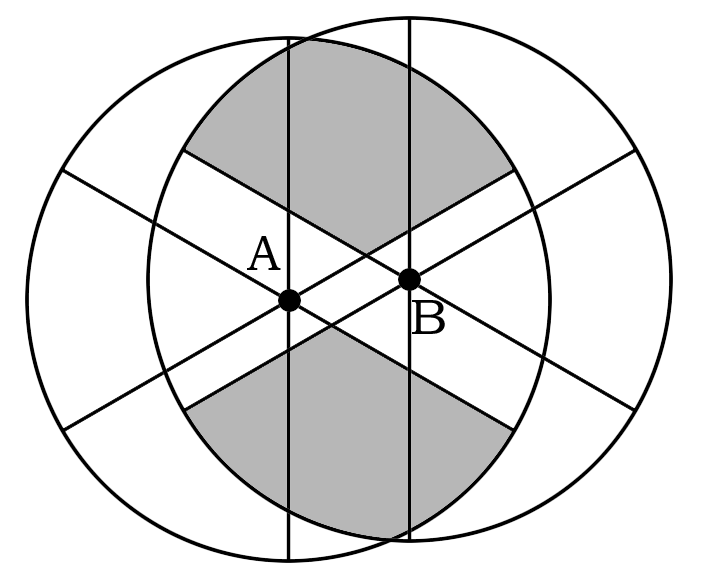
\includegraphics[width=5cm]{verifier-loose}
  \caption{Löyhällä paikkavaatimuksella}
  \label{fig:sub1}
\end{subfigure}%
\begin{subfigure}{.5\textwidth}
  \centering
  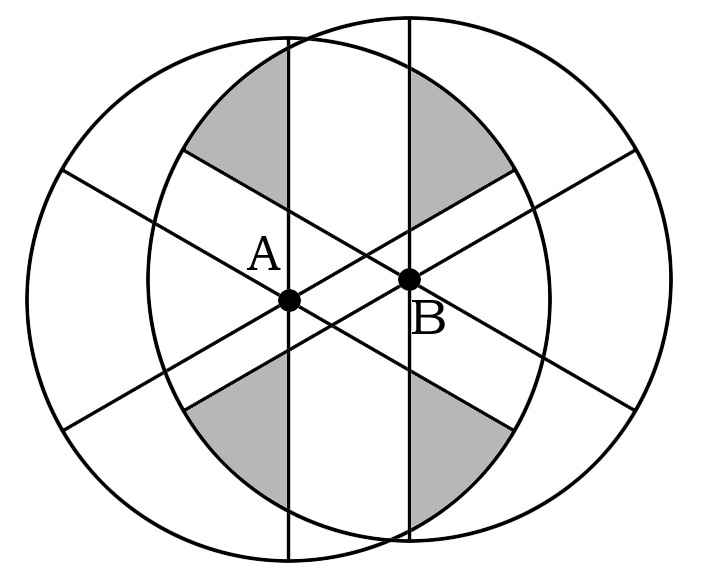
\includegraphics[width=5cm]{verifier-strict}
  \caption{Worawannotai-hyökkäyksen esteenä}
  \label{fig:sub2}
\end{subfigure}%
\caption{Todentajalaitteen mahdolliset sijainnit}
\label{fig:test}
\end{figure}


\subsection{SECTOR ja MAD}

SECTOR on kokoelma toimia, joilla voidaan todentaa laitteiden tapaaminen, ja MAD on protokolla, jolla voidaan suojautua madonreikähyökkäyksiä vastaan. Nämä molemmat kuvaillaan Capkunin, Buttyanin ja Hubaux'n artikkelissa ``SECTOR: Secure Tracking of Node Encounters in Multi-hop Wireless Networks'' \cite{sector}.

\paragraph{SECTORin oletukset järjestelmän ja verkon suhteen}
\noindent \\
Käyttöympäristönä voi toimia sekä puhdas mobiilien päätelaitteiden ad hoc -verkko että hybridimalli, jossa on paikoittain paikallaan olevia tukiasemia. 

\noindent \\
SECTORiin liittyy aikasidonnaisia osia, joten oletetaan kaikien laitteiden olevan varustettu kellolla. Koska operaatiot eivät ole yhtä tarkkoja kuin edellisessä protokollassa, riittää kellojen synkronointitarkkuudeksi alle sekunnin tarkkuus -- vertaa luvun~\ref{packetleashes} aikahihnojen satojen nanosekuntien tarkkuus. Vaikka synkronointi suoritetaan melko pienellä tarkkuudella, oletetaan ajanmittauksen tarkkuudeksi kuitenkin nanosekuntiskaalaa, jotta voidaan laskea kahden tapahtuman välissä kulunutta aikaa tarkasti ja tehdä sen perusteella päätöksiä.

\noindent\\
MAD-protokolla olettaa päätelaitteissa olevan lisälaitteen, joka osaa vastata verkon yli tulevaan bittihaasteeseen itsenäisesti ohittaen laitteen prosessorin.

\noindent\\
SECTOR olettaa myös, että verkossa on jokin keskitetty auktoriteetti, joka kontrolloi verkkoon liittymistä ja antaa laitteille uniikin identiteetin. Lisäksi oletetaan, että laitteilla on parikohtaiset salaiset avaimet tai toistensa todennetut julkiset avaimet. Tämä avainten jakaminen voidaan saada aikaan esimerkiksi tallentamalla avaimet verkkoa rakentaessa manuaalisesti laitteisiin tai käyttämällä jotakin avainvaihtoprotokollaa.

\paragraph{SECTORin määrittämät roolit ja niiden tehtävät}
\noindent\\
SECTOR määrittelee kolme eri roolia, joilla on omat tehtävänsä ja jokaisella näistä on erilainen vaikutus tullessa kaapatuksi vihamielisiin toimiin.

\begin{description}
\item[Kohtaaja] on laite, joka väittää kohdanneensa jonkin toisen laitteen ennen, jälkeen tai tarkalleen jonakin tiettynä ajanhetkenä.
\item[Todistaja] on laite, joka voi todistaa joko kohtaamisen ajanhetken -- jos todistaja itse oli kohdattu laite -- tai kohtaajan sijainnin tiettynä ajanhetkenä -- jos todistaja on havainnut laitteen.
\item[Varmentaja] on laite, jolle annetaan tiedot kohtaajan väitteestä ja todistajan tarjoama lisäinformaatio ja se pystyy tarkistamaan tietojen yhteensopivuuden ja täten varmentaa kohtaamisen tapahtuneen.
\end{description}

\noindent\\
Puhtaissa ad hoc -verkoissa, joissa laitteet ovat yhdenvertaisia, kaikki laitteet voivat toimia kaikissa rooleissa ja täten laitteiden väliset kohtaamiset voidaan joustavasti varmentaa minkä tahansa laitekolmikon toimesta. Mikäli käytössä on tukiasemallinen hybridiverkko -- kuten monihyppyinen matkapuhelinverkko -- voi varmentajana toimia vain osa verkon laitteista: tukiasemat.

\paragraph{MAD-protokolla}
\noindent\\
MAD-protokolla, eli molemminpuoleinen todennus etäisyysrajauksella (Mutual Authentication with Distance-Bounding, MAD), on hyvin yksinkertainen rakenteeltaan ja samalla varma tapa todentaa kahden laitteen tapaaminen. Protokollan ydinkomponentit ovat laitekohtainen satunnainen bittisarja sekä laite, joka voi autonomisesti ottaa vastaan yksibittisen haasteen ja lähettää takaisin XOR-bittioperaation tuloksen tästä bittihaasteesta ja laitteen satunnaisen bittisarjan seuraavasta bitistä.

\noindent\\
Protokollan alustusvaiheessa molemmat laitteet luovat \emph{l}-bittisen satunnaisen bittijonon sekä \emph{l'}-bittisen satunnaisen vahvistusbittisarjan. Aloitteen tehnyt laite, \emph{A}, lähettää tiivisteen näiden bittisarjojen yhdisteestä ja vastaanottaja, \emph{B}, lähettää vastaavan tiivisteensä takaisin. Bittisarjojen luonnin voi hoitaa jo ennen laitteiden kohtaamista, jotta laskentavaatimukset protokollalle kohtaamistilanteessa saadaan pienennettyä.

\noindent\\
Alustusvaiheen jälkeen laitteet aloittavat tuon \emph{l}-bittisen jonon läpikäynnin bitti kerrallaan. \emph{A} lähettää ensimmäisen bittinsä sellaisenaan ja tallentaa lähetysajan kellonsa maksimitarkkuudella talteen. \emph{B}:n bittihaastelaite laskee XOR-bittioperaation vastaanotetusta bitistä sekä sen seuraavasta, eli ensimmäisestä, bitistä, lähettää sen \emph{A}:lle sekä tallentaa oman lähetysaikansa. \emph{A} vastaanottaa \emph{B}:ltä tulleen vastauksen ja, kuten edellä, laskee XOR-bittioperaation seuraavan bittijononsa bitin kanssa ja lähettää sen. Tämän bittivaihdon lisäksi sekä \emph{A} että \emph{B} vertailevat paketin saapumisaikaa edellisen oman pakettinsa lähetysaikaan ja saavat täten sisäisen kellonsa tarkkuudella maksimietäisyyden välimatkalleen, koska paketti ei voi kulkea valonnopeutta nopeammin -- sama periaate kuin luvun~\ref{packetleashes} aikahihnojen kanssa.

\noindent\\
Kun \emph{l}-bittinen jono on kulutettu loppuun, seuraa protokollan varmennusvaihe, jossa molemmat osapuolet laskevat XOR-bittioperaatioilla alkuperäisen vastapuolen bittijonon ja laskevat siitä tiivisteen omien tunnistetietojensa kanssa sekä luovuttavat alustusvaiheessa lasketun \emph{l'}-bittisen jonon. Näiden tietojen avulla molemmat laitteet voivat päästä varmuuteen, että paketteja ei ole välissä muokattu.

\paragraph{Kohtaamisen ajankohdan todistustavat}
\noindent\\
SECTOR sisältää viisi erilaista tapaa todistaa kohtaamisen ajankohtaa. Nämä tavat on luokiteltu kahteen kategoriaan todistettavan ajankohdan tarkkuuden mukaan: kohtaamisen tuoreustakuu ja kohtaamisen aikatakuu. Tuoreustakuu takaa kohtaamisen tapahtuneen ennen tiettyä ajankohtaa, mutta ei todista ajankohtaa tarkasti. Kohtaamisen aikatakuu pystyy todistamaan ajankohdan halutulla tarkkuudella, joka on ennaltamäärätty. 

\paragraph{Kohtaamisen tuoreustakuu (Guaranteeing Encounter Freshness, GEF)}
\noindent\\
Tuoreustakuuta varten SECTOR määrittelee kaksi takuutasoa: todistaja-takuun sekä todistaja--kohtaaja-takuun. Ensimmäisessä jokainen verkon laite on etukäteen luonut satunnaisen luvun \emph{V} ja ottanut siitä \emph{N} rekursiivistä tiivistettä. N on etukäteen määritelty luku, jonka pitäisi kattaa kaikki tarvittavat todistuskerrat. Julkisena allekirjoituksenaan laitteet julkaisevat N:nnen rekursiivisen tiivisteen ja paljastavat edellisiä tiivisteitä ketjussa aika- tai pyyntöpohjaisesti. Koska protokolla olettaa tiivistefunktion olevan alkukuvaresistentti, tämä on yksinkertainen tapa todentaa laitteen olevan tiivisteketjun omistaja.

\noindent\\
Kohtaaja, \emph{A}, saa siis tällaisen kohdatun laitteen, \emph{B}, vielä paljastushetkellä kaikille tuntemattoman edellisen alkukuvan ja pystyy täten todistamaan varmentajalle kohtaamisen tapahtuneen. Tämä kuitenkin vain todistaa, että joku laite verkossa on tavannut \emph{B}:n ja \emph{A} on voinut vain kaapata tuon tiedon matkalla ja käyttää sitä hyväkseen nyt. 
\noindent\\
Tätä haastetta varten SECTOR tarjoaa todistaja--kohtaaja-takuun, jossa kaikki verkon laitteet luovat kaikkia muita verkon laitteita varten omat tiivisteketjunsa ja julkaisevat kaikkien tietoon omat juurensa jokaista eri laitetta varten. Täten laite \emph{M} ei voi käyttää laitteen \emph{A} saamaa alkukuvavastausta \emph{C}:ltä, koska \emph{C} on julkaissut kaikille sekä juuritiivisteen \emph{M} että \emph{A} varten ja jos tuota alkukuvavastausta käytetään rekursiivisesti tiivistefunktion läpi ei päädytä \emph{C}:n juuritiivisteenseen \emph{M}:lle.
\noindent\\
Tällaisen $n*(n-1)$ tiivistelistan ylläpito ei ole tilavaatimuksiltaan järkevää ottaen huomioon laitteiden rajalliset resurssit. Tämän lisäksi tuoreustakuu takaa vain tapaamisen tapahtuneen ennen tietyn avaimen paljastusta ja tilarajoitteiden takia noita avaimia ei voi luoda esimerkiksi joka sekunnille joten etäisyystarkkuus heikkenee.

\paragraph{Kohtaamisen aikatakuu (Guaranteeing the Time of Encounter, GTE)}
\noindent\\
Koska tuoreustakuun tarkkuus kohtaamisen ajankohdan suhteen ei ole riittävä, SECTOR kuvailee tähän tarkoitukseen paremman ratkaisun: samanlaiset Merkle-puut kuin luvun \ref{tik} TIK-protokollassa. Tässäkin Merkle-puun lehtisolmujen arvo on aikaan sidottu ja sen arvo muodostuu satunnaisluvusta. Kuten tuoreustakuussa on aikatakuussa samat takuutasot: todistaja-takuun sekä todistaja--kohtaaja-takuun. Nämä takuutasot oletuksena mukailevat tuoreustakuun toimintaa eli todistaja-takuuta varten jokaisella laitteella on yksi muodostettu Merkle-puu, jonka juuritiiviste toimii sen julkisena allekirjoituksena, ja todistaja--kohtaaja-takuuta varten jokainen laite luo jokaista verkon muuta laitetta varten oman tiivistepuun.

\noindent\\
Aikatakuun tapauksessa SECTOR tarjoaa kuitenkin myös optimoidun tavan tallentaa nuo kaikkien laitteiden tiivistepuut yhdeksi tiivistepuuksi per laite, jotta ei tarvitse jaella kuin yksi juuritiiviste. Tällöin jokainen laite muodostaa oman tiivistepuunsa, mutta ne ovat isomman tiivistepuun lapsia, katso kuva~\ref{fig:sectortrees}.

\begin{figure}
  \centering
  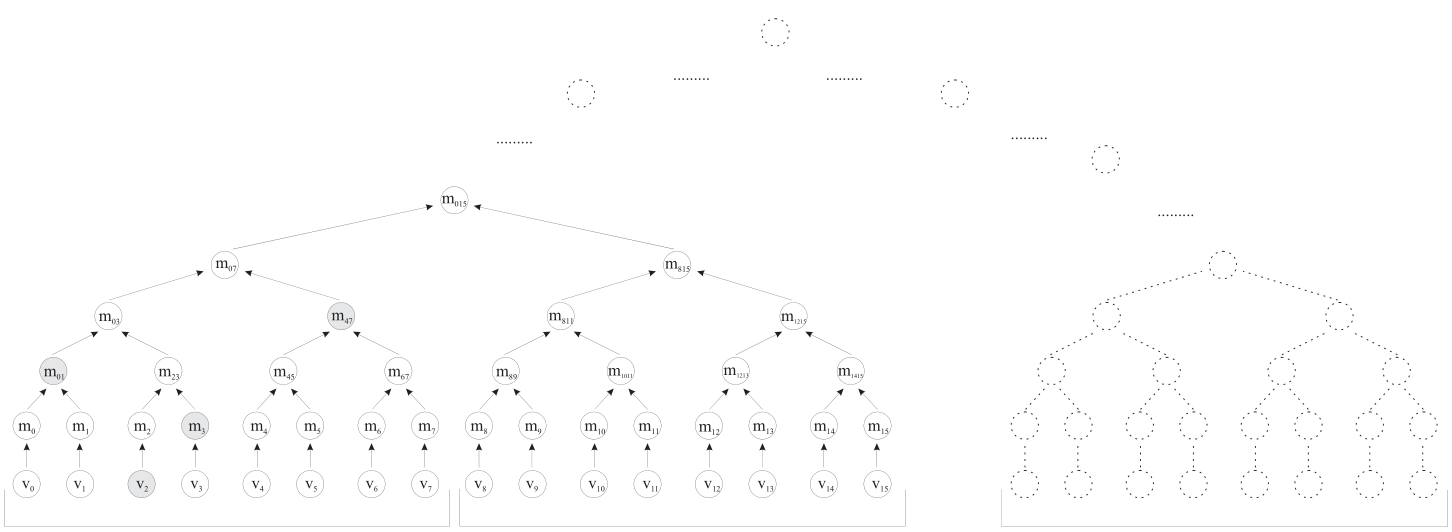
\includegraphics[width=\textwidth]{tree-of-trees}
  \caption{Kohtaamisen aikatakuuta varten muodostettava optimoitu tiivistepuiden tiivistepuu \cite{sector}}
  \label{fig:sectortrees}
\end{figure}


\noindent\\
Kuten luvun~\ref{tik} TIK-protokollassa, perustuu tiivistepuilla varmennus siihen, että jokaisen varmennuksen yhteydessä puun omistaja luovuttaa kaikki ne tiivistepuun solmut, jotka tarvitaan juuritiivisteen laskuun.

\paragraph{Hyökkääjien tyypitys}

\begin{description}
\item[Kohtaaja] Vihamielinen laite toimii Kohtaajan roolissa.
\item[Todistaja] Vihamielinen laite Todistajana.
\item[Kohtaaja-Todistaja] Vihamielinen laite molemmissa rooleissa
\item[Tarkistaja] Vihamieinen laite yrittää kerätä tietoa Kohtaajalta jotta voi saada Todistajan luulemaan tavanneensa Kohtaajan.
\end{description}

\paragraph{SECTOR-mekanismien toiminta hyökkäätyyppejä vastaan}

\begin{itemize}
\item GEF-Ce ja GTE-Ce
\item GEF-Ce ja GTE-Ce MAD-protokollan kanssa
\item GEF-CeCl ja GTE-CeCl MAD-protokollan kanssa
\item Julkisen avaimen ja symmetrisen avaimen -mekanismit
\item Muut hyökkäykset
\end{itemize}

\paragraph{Tila-, laskenta- ja viestintävaativuudet}

Tähän ehkä taulukko eri variaatioiden vaativuuksista käännettynä kirjoittajien taulukosta.

\section{Puhtaasti protokollapohjaiset puolustukset}
Seuraavilla ratkaisuilla on laajempi käyttöpotentiaali, koska ne eivät vaadi erityislaitteistoa.

\subsection{DeWorm}

Hayajneh et al kuvailevat DeWorm-protokollan \cite{deworm}, jonka mainitaan erityisesti olevan tehokas \emph{piilotettuja hyökkääjiä} vastaan -- eli madonreikähyökkääjät M1 ja M2 siirtävät paketteja keskenään eivätkä itse osallistu verkon laitteina reititykseen.

\paragraph{Perusajatus}
\noindent \\
Kun laite A haluaa selvittää onko sen ja laitteen B välissä madonreikä, se aloittaa DeWorm-protokollan mukaisen vaihtoehtoisen reittihaun: jokaiselle noodille polulla A--B katsotaan, että sitä seuraavasta seuraavaan noodiin vievän reitin pisimmän ja lyhimmän siirtymän pituuksien erotus ei ole raja-arvoa $n$ suurempi. 

\noindent \\
Esimerkki: A--B väli on kokonaisuudessaan A-1-2-3-4-B. A pyytää kaikilta naapureiltaan löytämään reitin noodiin 2 siten että reitti ei kulje nykyisen reitin kautta eli noodin 1 läpi. Reitti A--2 on kahden hypyn pituinen; jos löytyy yksi tai useampi reitti, jonka pituus on $2 + n$ tai enemmän, A olettaa välillä A--2 olevan madonreikä. Mikäli madonreikää ei löydy, seuraavaksi tarkistetaan 1--3 ja taas pyydetään 1:n naapureita löytämään reitti 3:een kulkematta noodin 2 kautta. Tätä jatketaan kunnes erikoistapauksena käsitellään toiseksi viimeinen noodi (4), joka pyytää kaikkia naapureitaan löytämään reitin B:hen kulkematta itsensä läpi. Mikäli missään vaiheessa ei ole löytynyt raja-arvoa $n$ suurempia poikkeamia reittien pituuksissa, voi A olla varma ettei matkalla ole madonreikää.

\paragraph{Ongelmat}
\noindent \\
Raja-arvon $n$ valinta kriittistä, jotta voidaan tasapainotella virheellisten tunnistusten ja tunnistamatta jättämisen välillä. Kirjoittajien simulointien perusteella he suosittelevat $n$ arvoksi 2--3.

\noindent \\
Toinen ongelma on niin sanotut kriittiset solmut, eli laitteet jotka legitiimisti yhdistävät kaksi verkkoa ainoana solmukohtana. Tällainen solmukohta näyttää DeWorm-protokollan silmin madonreiältä ja siksi verkon pitää pystyä ottamaan tällainen huomioon esimerkiksi antamalla kriittiselle solmulle ja sen naapureille erivapauden DeWorm-protokollan ohitukseen. Tällainen erivapaus on mahdollista sallia, koska DeWorm-protokolla on suunniteltu ja testattu liikkumattomiin verkkoihin, joissa verkon muoto on tiedossa etukäteen.

\noindent \\
Viimeisimpänä ongelmana on protokollan suuri liikennemäärä: jokainen verkon noodi voi päätyä tarkistamaan madonreikien olemassaolon jokaiseen noodiin, jonka kanssa se on yhteydessä. Kirjoittajat eivät kuitenkaan kuvaile, miten laitteen pitäisi päättää aloittaa DeWorm-protokollatarkistus.

\subsection{DelPHI}

Hon Sun Chiu ja King-Shan Lui kertovat viiveeseen perustuvasta DelPHI-protokollastaan \cite{delphi}. Koko protokollan ydinajatus on hyvin yksinkertainen: verkon jokaisen hypyn pitäisi olla pituudeltaan suunnilleen yhtä pitkä ja täten madonreiän voi löytää havaitsemalla reitin, jonka lähetysaika per hyppyjen määrä on suuri. Normaali reitti verkon poikki etenee tasaisin hyppäyksin, joita voi olla melko montakin verkon laidalta toiselle, mutta madonreiässä liikutaan pitkä fyysinen matka yhden hypyn aikana. Tällöin tuo yksi hyppy erottuu selkeästi hitaampana ja täten epäilyttävänä.

\paragraph{Esimerkki}

\noindent\\
\begin{tikzpicture}
  [scale=.8,auto=left,every node/.style={circle,fill=gray!20}]
  \node (A) at (10,8)  {A};
  \node (B) at (12,8)  {B};
  \node (C) at (14,8)  {C};
  \node (D) at (16,8)  {D};
  \node (E) at (18,8)  {E};

  \foreach \from/\to in {A/B,B/C,C/D,D/E}
    \draw (\from) -- (\to);

\end{tikzpicture}

\noindent\\
Pituus A--E: 4 hyppyä. Aikaa kuluu $T_1$.

\noindent\\
\begin{tikzpicture}
  [scale=.8,auto=left,every node/.style={circle,fill=gray!20}]
  \node (A) at (10,8)  {A};
  \node (M1) at (12,8)  {(M1};

  \node (M2) at (16,8)  {M2)};
  \node (E) at (18,8)  {E};

  \foreach \from/\to in {A/M1,M1/M2,M2/E}
    \draw (\from) -- (\to);

\end{tikzpicture}

\noindent \\
Pituus A--E: 1 hyppy M1 ja M2 ollessa \emph{piilotettuja hyökkääjiä}. Aikaa kuluu: $T_2$.

\noindent \\
Koska molemmissa esimerkeissä signaali kulkee maksimissaan valonnopeutta ei kokonaisaika todennäköisesti ole kovin paljon erilainen, eli $T_1 \approx T_2$ ja täten $(T_1 / 4) < (T_2 / 1)$ vaikka tämä reitti olisi pituutensa puolesta muuten parempi.

\paragraph{Protokollan eteneminen}
\noindent \\
\emph{Vaihe I}: Laite A aloittaa DelPHI-madonreikätunnistuksen lähettämällä DREQ-tietoliikennepaketin B:lle yleislähetyksenä. Koska paketti lähtee yleislähetyksenä, kaikki A:n naapurit kuulevat paketin ja tallentavat oman tunnisteensa paketin \emph{edellinen hyppy} -kenttään, kasvattavat hyppymäärälaskuria ja lähettävät sen yleislähetyksenä eteenpäin. Kun DREQ-paketti vihdoin saapuu B:lle, se lähettää vastauksena DREP-tietoliikennepaketin jokaista vastaanottamaansa DREQ-pakettia varten suoraan A:lle. Nämä DREP-paketit palaavat tulemaansa reittiä pitkin ja A saa tietää useita uniikkeja reittejä verkon läpi.

\noindent \\
\emph{Vaihe II}: Saatuaan vastaukset DREQ-pyyntöönsä laite A voi analysoida reittien pituuksien suhteita keskiarvoiseen hypyn viiveeseen. Mikäli näiden eri hyppyviiveiden välinen ero ylittää raja-arvon $T$, voi A olettaa madonreiän reitille. Kirjoittajien analyysin perusteella madonreikähyökkäyksen yhteydessä nämä hyppyviiveet jakautuvat kahteen ryhmään siten, että kahden ryhmän välillä oleva aikaero on aina suurempi kuin ryhmän sisäinen hajonta. 

\noindent \\
Esimerkkiarvoina tuolle raja-arvolle $T$ annetaan 1-5 millisekuntia. Arvon ollessa 1 ms tunnistuu osa (15--20\%) valideista reiteistä madonrei'iksi ja madonrei'istä tunnistetaan suurin osa (65--97\%). Raja-arvolla 5 ms väärien tunnistusten arvo on marginaalista (1--3\%) ja madonrei'istä tunnistetaan simulaatioverkon koosta riippuen noin 10--89\%. Simulaatioverkkojen koko vaikutti merkitsevästi tunnistustarkkuuteen: raja-arvoilla 1--5 ms tunnistustarkkuus vaihteli pienemmässä verkossa 65--10,4\% ja kaksinkertaisen kokoisessa verkossa 97,6--89\%.


\subsection{LiteWorp}

Khalil et al esittelevät naapurilistoihin ja vartiointiin perustuvan LiteWorp-protokollan \cite{liteworp}. Protokollan oletuksina on verkon staattisuus -- laitteet eivät siis liiku -- ja laitteilla olevan parien välinen jaettu avain.

\paragraph{Verkkoon liittyminen}
\noindent \\
A:n liittyessä verkkoon se lähettää yleislähetyksenä tiedon olemassaolostaan. Kaikki viestin kuulijat vastaavat A:lle todentaen vastauksensa heidän yhteisellä jaetulla avaimellaan. A lisää kaikki todennetun vastauksen lähettäneet laitteet naapurilistaansa, $R_A$. Kun A:n yleislähetyksen aikaraja on mennyt, se lähettää kaikille naapureilleen oman naapurilistansa todentaen viestinsä jokaiselle erikseen jaetulla avaimella. Täten liittymisen yhteydessä A tietää naapurinsa ja A:n naapurit tietävät kaikki A:n naapurit.

\paragraph{Paikallinen valvonta}
\noindent \\
Koko protokollaan perusajatuksena on, että kaikki laitteet vartioivat kaikkea kuulemaansa liikennettä. Mikäli laite C saa laitteelta B paketin, jonka B sanoo tulevan A:lta mutta C:n tietojen mukaan A ei ole B:n naapuri, C hylkää paketin ja kohottaa B:n paha-aikeisuuslaskuria $Mal_B$ jonkin ennalta määrätyn \emph{tekaisulisäyksen} verran.

\noindent \\
Toinen rike, jota verkossa olevat laitteet valvovat, on pakettien tahallinen pudottaminen. Tätä varten jokainen verkon laite pitää jokaista kuulemaansa naapuria varten erillistä vahtilistaa paketeista, jotka naapurin olisi tarkoitus lähettää eteenpäin. 

\noindent \\
Alla olevan kuvaa esimerkkinä käyttäen M1:n saadessa paketin A:lta B:lle tekee laite C omaan vahtilistaansa merkinnän tästä paketista ja odottaa hetken verran että M1 lähettää paketin normaalisti eteenpäin B:n suuntaan. Mikäli C ei havaitse M1:n lähettäneen sille tullutta välitettäväksi tarkoitettua pakettia eteenpäin, korottaa C nyt $Mal_{M1}$-paha-aikeisuuslaskuria \emph{pudotuslisäyksen} verran.

\noindent\\
\begin{tikzpicture}
  [scale=.8,auto=left,every node/.style={circle,fill=gray!20}]
  \node (A) at (4,7)  {A};
  \node (B) at (8,7) {B};
  \node (C) at (6,9)  {C};
  \node (M1) at (6,7)  {M1};

  \foreach \from/\to in {A/M1,M1/B,A/C,B/C}
    \draw (\from) -- (\to);

\end{tikzpicture}

\paragraph{Eristäminen}
\noindent \\
Kun C on havainnut raja-arvon, $C_t$, verran rikkeitä M1 toimesta, se poistaa M1:n omalta naapurilistaltaan ja lähettää kaikille M1 naapureille tiedon siitä, että epäilee M1:stä paha-aikeiseksi laitteeksi. Kaikki M1:n naapurit tarkistavat, että C on ollut M1:n vartija, ja merkkaavat C:n omaan varoituspuskuriinsa M1:n suhteen. Laitteen saadessa luottamusrajan, $\gamma$, ylittävän määrän varoituksia M1:stä se poistaa M1:n omalta naapurilistaltaan. Tämän luottamusrajan asettaminen liian alhaiseksi voi luoda tilanteen, jossa verkon normaalit laitteet voivat joutua väärin leimatuksi ja verkosta hylätyksi. Liian korkea luottamusraja voi johtaa paha-aikeisten laitteiden huomaamatta jäämiseen. Nämä varoitukset ovat tosiaan kumulatiivisia eikä niissä ole aikarajaa.

\paragraph{Analyysia toimivuudesta}
\noindent \\
Yksi tämän protokollan toimintavarmuuteen vaikuttavista tekijöistä on verkkotason pakettitörmäykset. Törmäyksistä voi aiheutua se, että vartijalaite ei havaitse vartioimalleen laitteelle tullutta välitettävää pakettia ja laitteen vartioitavan lähetettäessä tämän paketin normaalisti eteenpäin vartijalaite katsoo tämän tekaisseen paketin. Vaihtoehtoisesti pakettitörmäys voi peittää vartijalta näkyvyyden paketin oikeaan edelleenvälitykseen ja täten viattoman laitteen paha-aikeisuuslaskuria kohotetaan \emph{pudotuslisäyksellä} vaikka se oikeasti lähetti paketin.

\noindent \\
Kirjoittajien analyysin perusteella todennäköisyys madonreiän tunnistamiselle verkossa riippuu naapureiden määrästä. Alle 7 naapurin verkoissa protokolla ei toimi, mutta 7 naapurilla todennäköisyys madonreiän tunnistamiseen on noin 90\% ja se kohoaa 100\%:iin jo 11 naapurilla. Yhteentörmäysten takia protokollan teho alkaa heikentyä liian täydessä verkossa: yli 20 naapurin verkoissa todennäköisyys tunnistuksella putoaa lähes lineaarisesti siten että 35 naapurin verkossa todennäköisyys on enää noin 40\%.

\noindent \\
Vaikka väärien tunnistusten mahdollisuus on jo tuotu esille, ei se todellisuudessa kirjoittajien mukaan ole kovin suuri uhka. Pahimmillaan todennäköisyys legitiimin laitteen väärään tunnistukseen paha-aikeisena 23 naapurin verkossa on 0,00003\%.

\subsection{MobiWorp}

Khalil et al jatkavat LiteWorpin ideaa staattisista verkoista mobiileihin verkkoihin MobiWorp-protokollallaan \cite{mobiworp}.

\noindent \\
Perusidea vartijoista ja naapurilistoista yhä sama, nyt lisänä laitteiden liikkumiseen liittyvät protokollaosat.

\begin{itemize}
\item Selfish Move Protocol (SMP)

\end{itemize}

\section{Yhteenveto}

Madonreikähyökkäys on erittäin vakava uhka langattomissa ad hoc -verkoissa. Siitä tekee erityisen kavalan se, ettei hyökkääjien tarvitse murtaa minkäänlaista salausta vaan ne voivat saada haittaa aikaan puhtaasti verkkokerroksella paketteja kopioiden verkon osien välillä. Tästä seuraa se, että suuri osa puolustuskeinoista perustuu arvioimaan toimivatko muut laitteet ja verkkopolut joidenkin ennalta asetettujen raja-arvojen puitteissa. Nämä raja-arvot päättävät sen löytyykö verkosta kaikkien hyökkääjänoodien lisäksi myös viattomia laitteita väärin tunnistettuina vai jääkö osa hyökkääjistä epäilyttä.




% --- References ---
%
% bibtex is used to generate the bibliography. The babplain style
% will generate numeric references (e.g. [1]) appropriate for theoretical
% computer science. If you need alphanumeric references (e.g [Tur90]), use
%
%
% instead.
\newpage

%\bibliographystyle{babplain-lf}
\bibliographystyle{babalpha-fl}
\bibliography{references-fi-full}


% --- Appendices ---

% uncomment the following

% \newpage
% \appendix
% 
% \section{Esimerkkiliite}

\end{document}
